\newpage
\section{Tecnologie utilizzate}
	L'obbiettivo di questo paragrafo è quello di descrivere in modo generale come il prodotto andrà ad interfacciarsi con le tecnologie che avranno il ruolo di producer e consumer in modo tale da ricevere le notifiche e inoltrarle in maniera corretta al destinatario più adeguato.
	Di seguito un'immagine presa dalla presentazione del capitolato che rappresenta lo scopo del prodotto finito:
	\vspace{-0.4cm}
	\begin{figure}[H]
		\centering
		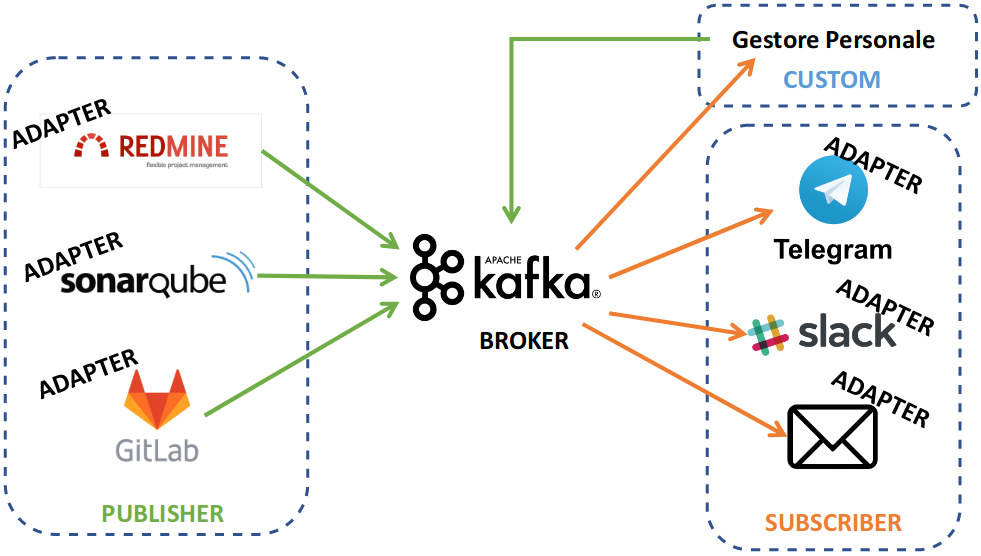
\includegraphics[width=\columnwidth]{img/butterfly.png}\\
		\caption{Rappresentazione della comunicazione tra publisher e subsriber passando per il broker}
	\end{figure}

	Per ciascuna tecnologia con cui l'applicativo andrà ad interfacciarsi è previsto un microservizio, il quale avrà come scopo quello di fare da tramite.

	\subsection{Producers}
		In ordine di priorità richiesta dal committente, i software che svolgono il ruolo di producer sono:

		\subsubsection{Redmine}
		Ciascuna istanza di Redmine permette l'utilizzo delle proprie API con le quali potersi interfacciare e ricevere risposte nel formato scelto.
		Queste vengono prese dal server tramite un microservizio facente parte dell'applicativo che ne fa la richiesta ad intervalli determinati prestabiliti aggiornando in base a quello che riceve i dati presenti sul gestore personale e inoltrando le notifiche ai customer interessati.
		%http://www.redmine.org/projects/redmine/wiki/Rest_api
		
		\subsubsection{GitLab}
		Ciascuna istanza di GitLab (online o in un server interno dell'azienda) mette a disposizione la configurazione di webhooks che, alla modifica della repo, manda un messaggio con le informazioni aggiornate e il cambiamento che è avvenuto a un microservizio capace di aggiornare i dati presenti nel gestore personale e, come prima, inoltrare le notifiche ai customer interessati.
		%https://docs.gitlab.com/ee/user/project/integrations/webhooks.html
		
		\subsubsection{SonarQube}
		Come GitLab, anche SonarQube prevede l'utilizzo di webhooks che dopo ciascuna build manda le il risultato e le informazioni relative ad un microservizio capace di aggiornare i dati presenti nel gestore personale e, anche in questo caso, inoltrare le notifiche ai customer interessati.
		%https://docs.sonarqube.org/latest/project-administration/webhooks/
		
	\subsection{Broker}
	
		L'azienda consiglia di utilizzare come broker per i messaggi Apache Kafka.
	
		\subsubsection{Apache Kafka}
		
		
	
	\subsection{Consumers}
	
		In ordine di priorità richiesta dal committente, i software che svolgono il ruolo di producer sono:
	
		\subsubsection{Telegram}
		Telegram permette l'interazione in maniera automatica con gli utenti tramite bot che possono essere configurati per mandare messaggi ricevuti da strumenti di terze parti, come in questo caso il broker apache kafka.
		%https://core.telegram.org/bots
		
		\subsubsection{E-mail}
		Per l'invio delle mail agli utenti finali è necessaria la configurazione di un server di posta interno, che sfrutta quindi il protocollo SMTP, in modo tale da poter mandare mail con le informazioni richieste ai customer interessati.
		%https://realpython.com/python-send-email/
		
		\subsubsection{Slack}
		È possibile utilizzare le API di Slack per poter mandare push notifications ai canali o alle persone interessate specificando il nome del canale (o lo username della persona), testo del messaggio, e lo username che verrà mostrato per il mittente.
		%https://www.confluent.io/blog/real-time-syslog-processing-with-apache-kafka-and-ksql-part-2-event-driven-alerting-with-slack/
	
	\subsection{Gestore personale}
	Il gestore personale è quello che permette agli utenti di impostare le proprie preferenze per il canale di inoltro dei messaggi ed i topic a cui si iscrivono interfacciandosi dunque con l'intero sistema.
	È previsto come un'applicazione web installata in un server interno all'azienda accessibile dai dipendenti interessati che potranno quindi modificare (con la possibilità di aggiungere e togliere) impostazioni come topic a cui si è iscritti e modalità di ricezione dei messaggi.
	
	\subsection{Container Software}
	
		Un container software simula questo ambiente virtuale dove è possibile testare e mantenere le proprie applicazioni, permettendo di aumentare l'efficienza riducendo i costi e simulando un computer su una macchina con risorse condivise.
		
		\subsection{Differenza tra container e macchina virtuale}
		A differenza delle macchine virtuali, dove lo stato dell'ambiente viene salvato su disco occupando memoria, i container si adattano in maniera migliore all'applicativo richiesto in quanto il loro scopo è quello di massimizzare la quantità delle applicazioni in esecuzione riducendo al minimo il numero delle macchine.
		Sono quindi più leggeri, occupando meno memoria su disco e impiegando meno risorse, però al termine della loro esecuzione non viene salvato lo stato, a meno che non sia esplicitamente richiesto.
		
		
		\subsubsection{Docker e Dockerfile}
		L'azienda consiglia di utilizzare Docker per la semplicità e perché si adatta all'architettura con i microservizi.
		La configurazione avverrà tramite un dockerfile in cui verranno specificate informazioni come sistema operativo, script all'avvio, numero di istanze ed altri parametri specifici.
			
	\subsection{Protocolli per API}
	https://searchmicroservices.techtarget.com/definition/REST-representational-state-transfer